\documentclass [a4paper, 10pt]{article}

\usepackage[ansinew]{inputenc}
\usepackage[danish,english]{babel}
\usepackage{amsmath,amssymb,amsfonts}
\usepackage{verbatim}
\usepackage{graphicx}
%\usepackage{fancyhdr}
%\usepackage[pdftex,bookmarksnumbered,colorlinks,backref, bookmarks, breaklinks, linktocpage]{hyperref}

\frenchspacing \setlength{\parindent}{0pt}
\setlength{\parskip}{1ex plus 0.5ex minus 0.2ex}

\addtolength{\textwidth}{1cm}
\addtolength{\textheight}{1cm}

\setlength{\parindent}{0pt} % for adjusting indentation

\hyphenation{desirable finally sta-ti-sti-cal-ly basic tailored}

\title{Green Wave Traffic Optimization -- A Survey}
\author{Andreas Warberg,\\ Department of Transport, Technical University of Denmark\\ ~ \\ 
Jesper Larsen,\\ Department of Management Engineering, Technical University of Denmark\\ ~ \\ Rene Munk J{\o}rgensen,\\ Department of Transport, Technical University of Denmark}
\date{\today}

\begin{document}

\setlength{\parindent}{4mm}

\maketitle

\begin{abstract}
The objective of this survey is to cover the research in the area of
adaptive traffic control with emphasis on the applied optimization
methods.

The problem of optimizing traffic signals can be viewed in various
ways depending on political, economic and ecologic goals. The survey
highlight some important conflicts, which support the notion that
traffic signal optimization is a multi-objective problem, and relate
this to the most common measures of effectiveness.

A distinction can be made between classical systems, which operate
with a common cycle time, and the more flexible, phase-based,
approach, which is shown to be more suitable for adaptive traffic
control. To support this claim three adaptive systems - not dependent
on a common cycle time - are described in detail."
\end{abstract}

\section{Introduction}

Road traffic is an essential part of modern society and has put a high
demand on road networks. Figures from a recent study from the Danish
ministry of transport \cite{47} shows traffic has increased by 50\%
since the 80's and that cars and busses are responsible for more than
90\% of all person transport in Denmark (totalling 68 milliom
kilometers).

Traffic network congestion causes delays which adds substantial costs
to the society and businesses on a daily basis and also increases
emissions and the risk of accidents. In the beforementioned study it
is reported that in 2002 people where spending 100,000 hours in total
in queue in the Greather Copenhagen road infrastructure, this
corresponds to an economic loss of more than 750 million Euros.  

To alleviate congestion, public transport can be improved or the
infrastructure can be expanded. In urban areas, the latter is often
impossible due to residential areas adjacent to the existing roads.
A more subtle way to improve the network performance is to make better
use of the existing roads, which can be done by proper setting of
traffic signal parameters.

It is estimated that the proper use of intelligent traffic systems
including intelligent traffic signals can increase the capacity of the
road network in the Greater Copenhagen area by 5 to 10\%.

Traffic signals are employed in urban areas in order to control
traffic flows and avoid collisions by fairly distributing the
right-of-way for adjoining road segments and to ensure a smooth flow
of traffic. If not set appropriately traffic signals may seriously
affect the traffic flow through the road network and so great care
should be taken when choosing the parameters for an intersection.

The literature has many suggestions for the intelligent setting of
traffic signals, ranging from purely statistically based methods
developed in the early 60's over actuated traffic signals to highly
adaptive and cooperative methods, which can be realized using actual
flow information supplied by traffic detectors. This paper gives a
survey of the literature with special emphasis on adaptive methods,
which attempts to coordinate traffic signals in larger networks so as
to optimize some network-wide performance index such as number of
stops or delay.

The paper is structured as follows. XXX Oversigt skal skrive naar
resten er paa plads XXX. Finally in section \ref{sec:conclusion} we
summarize the findings and come with recommendations for future works.


\section{Definitions and setup}
\label{vocabulary}
There are many terms concerning traffic signal optimization. This section attempts to extract the most important terms and give solid descriptions.


\begin{description}

	\item[MOE] Measure Of Effectiveness. Also referred to as the performance index (PI).
	Most often used is the average delay, also common is the time in (traffic) network and number of stops. 
			
	\item[Cycle] The turnaround time for all phases of a traffic signal to complete.
	
	\item[Phase,] also referred to as \textit{stage} corresponds to a particular state of the red and green lights of the traffic lights in an intersection. 
	For instance there may be a green phase in the north and south direction for a two-way intersection (which implies red phase in the east-west direction).

\item[Interphase green,] or lost time, is a small amount of time inserted as a buffer between two phases. During the lost time the lights can be either red in all directions or, as in Denmark, amber lights can be used to introduce a buffer. The purpose of the buffer is to allow vehicles, which entered during the last phase, to exit the intersection before it is flooded by vehicles from the next phase.
	
	\item[Split] (Or \textit{cycle}-split) is the green-to-red time ratio split. Usually a higher ratio means more green time.
	
	\item[Traffic assignment] also known as flow assignment, is the determination of vehicular flow along origin-destination (OD) paths and, consequently, along links in a traffic network. 

\item[Artery] is a main-path through a traffic network. It will generally face higher demand than auxilliary paths.

\item[Traffic network] is most often described mathematically as a graph $G(V,E)$ where $V$ is the set of intersections controlled by a traffic signal and $E$ is the set of roads connecting the intersection. A path is thus a route through the network crossing a least one signalized intersection.

	\item[A platoon] is group of vehicles travelling together. A platoon can be detected by observing the time between on vehicle and the next and applying the critical headway threshold, see \cite[sct. 2]{25}. 
Platoons are formed both as a consequence of car-following behaviour, which is used in simulation frameworks such as \cite{treiber-2000-62}, but also due to the batch-like nature which is imposed on the traffic by traffic signals.

\item[Saturation flow rate] defines the number of vehicles that can free flow on a link during a period of time.

\item[Time horizon.] The amount of time into the future, which is taken into consideration while optimizing signal settings. Using a shorter time horizon the optimizations might prove to be flawed, but with longer time horizons the predictions of traffic become less accurate.

\item[Vehicle Actuated Programming] (VAP) is an optional add-on module for the
simulation of programmable, phase- or stage-based, and traffic-actuated signal controls in VISSIM.

\end{description}


%\section{Survey Objective \& Scope}
%\label{scope}
The objective of this survey is to cover the research into adaptive traffic control with emphasis on the applied optimization methods.

The survey was made from a collection of about 50 papers and research reports, which cover from static optimization of a single intersection to large-scale systems designed to coordinate multiple signals. 

In addition, to obtain some operational insight, two interviews was performed with danish road authorities. 

The first one was with \textit{Lars Bo Frederiksen} and \textit{Nicolai Ryding Hoegh} of Centre for Traffic. They control more than 350 signals in the municipality of Copenhagen including 2 systems for adaptive control (in Valby and at \textit{Centrumforbindelsen} resp.). 

The second interview was done with \textit{Steen Merlach Lauritzen} at the Danish Road Directorate. The Danish Road Directorate supervise the regional road infrastructure which is mostly freeways and highways. They have a number of adaptive control systems (MOTION by Siemens, UTOPIA/SPOT by Swarco, DOGS by Technical Traffic Solution).

This report will discuss such things as:

\begin{itemize}
\item The objective function and the inherent multi objectivity of the problem
\item Optimization types
\item Cooperation among signal controllers
\end{itemize}

It will not go into detail on e-conomic or safety issues nor will it discuss optimizations for soft trafficants. Detection is not investigated in detail; it is assumed that there exist solid solutions for detection and that the control software has good to near-perfect information about the state of the traffic network.


\section{Defining Performance}
\label{sec:theproblem}

Essential parameters to the performance of a signalized intersection
-- or network of intersections -- are cycle time, green split and the
offset related to the common cycle time.

The amount of consecutive green time, which can be distributed to the
phases of an intersection depends on the cycle time. This is why the
cycle time is very important to the chosen MOE. In \cite{41} Sun et
al. explain that 

\begin{quote}[...] minimizing delay leads to short cycle length while
minimizing stops indicates long cycle length.
\end{quote}

The reason is that a long cycle length may stop a whole group of
vehicles (also known as a platoon) and incur a large delay for them,
but the platoon of vehicles only experience a single stop. With short
cycle time the vehicles never have to wait long for a green light but
are on average stopped more frequently.

%% Most authors who consider coordination of multiple signals use and
%% optimize a cycle time which is common for all traffic signals since it
%% would otherwise become hard to coordinate signals in static
%% schedules. In a small network, if each signal operates on its own
%% cycle time, green waves would only work on a periodic basis when the
%% cycle time and offset parameters of all signals eclipse. Otherwise the
%% green wave would drift and either cut off platoons of vehicles or give
%% too much green time.

The cycle time of an intersection is one of the most important
parameters in a signal plan since it sets  lower and upper bounds on
the green times for the phases. This relates to the MOE as well as the
safety of a network since 1) if a red light is shown for too long some
motorists may start to ignore the signals and 2) if the signals
cycle too frequently there is an increased risk of collisions.

The green split, which is the green-time to cycle-time ratio for the
phases of the intersection, should be considered as an indication of
the amount of traffic expected from each road facing the
intersection. Major roads will be given the larger split and minor
roads a smaller split.

The offset for an intersection is used to accommodate green waves for
traffic travelling from intersection to intersection at a specified
pace. This parameter is mostly relevant when optimizing signal plans
for major-minor types of arterials where platoons travel (mostly)
along a path, which traverses a string of intersections. Some of the
most promising results for this specific type of optimization are from
MAXBAND and MULTIBAND, described in \cite{37}.

Almost all methods optimize some or all of these three parameters. A
less commonly optimized parameter is the \textit{phase sequence}
ie. the order in which phases should be green during a cycle. This is
mostly relevant when prioritizing certain types of traffic, eg. public
transport (see \cite{scoot2004}) or emergency vehicles, but also when
considering safety aspects.

The problem of choosing an MOE depends on, among other things:

\begin{itemize}
\item The type of traffic which should gain benefits: private and commercial vehicles, public transportation, pedestrians and cyclists.
\item The network: highway, rural, urban.
\item Political objectives: safety, priority to businesses, reduction of emmisions combined with more public transportation and \textit{green} buses, which run on alternative fuels.
\end{itemize}

Clearly there are conflicts of interest among this selection of
objectives. One example has already been mentioned. Other examples of
objective conflicts are:

\begin{itemize}
\item Minimizing delays for vehicles along an artery will cause longer waiting times for crossing pedestrians.
\item Prioritizing eg. public transport by skipping a phase will lower the performance for private transport. 

In the SCOOT system (see \cite{scoot2004}) a phase skipping approach
to bus prioritization was implemented and tested in a London
intersection. The buses enjoyed 4 sec less delay but the delay for
non-bus vehicles increased by 1 sec in total on average. The vehicles
on the roads with no bus traffic suffered up to 14 sec delay on
average, however.

\item Any optimization which improves the experience of traversing the network by vehicle will probably cause more traffic and thus increase emissions.

\end{itemize}

Most of the articles in the survey use the average delay as an
objective. The TRANSYT optimization package by Robertson (1969) uses
the performance index (same as MOE) as explained in \cite{26}:

\begin{quote}
The performance index is defined as the sum for all signal-controlled
traffic streams of a weighted linear combination of estimated delay
and number of stops per unit of time and is used to measure the overall
cost of traffic congestion associated with the traffic control plan.
\end{quote}

Thus TRANSYT faces the multi-objectivity but the weights must be
defined and maintained by the traffic engineers supervising the
system. This is not a trivial task and requires intimate knowledge of
the network as well as the optimization package. The TRANSYT manual
suggests that weights should be set so that 1 stop $\simeq$ 20 sec
delay. This is in line with the guidelines used by the Danish Road
Directorate (DRD).

In \cite{41} a true multi-objective optimization approach is
tested. Sun et al. use a Non-dominated Sorting Genetic Algorithm (NSGA
II) to find Pareto-optimal solutions for the minimization objectives
\textit{average delay} and \textit{number of stops} per unit of time.


\section{The Optimization Problem}
\label{model}
The problem is now formulated as the minimization of a selected performance index (PI) in terms of a set of signal settings, $\Psi$, and a network, which is dependent on the signal settings.

$$\min PI \left(  \Psi, N\left( \Psi\right)  \right)  $$

In a general, discrete time, model time each time steps are denoted by $t$. The network consists of $N \geq 1$ signal controlled intersections indexed by $n$.

In the model each signal is designated a phase for each time unit. Thus the concept of a cycle becomes virtual as they are no longer mandatory for calculating eg. the length of phases given the green splits.

Without a common cycle time - or individual cycle time, even - the offset parameter also disappears. However they can be made to exist virtually, in terms of a virtual cycle, and can thus be manipulated to excert the same behaviour. 
The main problem is during initialization when the system has just started. In this case it is possible synchronize intersections by delaying startup for those that would otherwise have a positive offset and vice versa for negative offset intersections. The same strategy can be used when increasing or decreasing the (virtual) cycle time for the arterial.

Phase sequences and green splits are unified by the specification of the phase in a timeslot, $t$, referred to as $p_n(t)$. For each intersection there will be a fixed number of phases, $P_n$, which are free from right-of-way conflicts. For a simple cross intersection with left-side driven vehicles (see figure \ref{fig:simple_intersection}) this number is 2: straight, left, and right turning flows in north and south directions for phase 1 and in east and west directions for phase 2.

\begin{figure}[!h]
\begin{center}
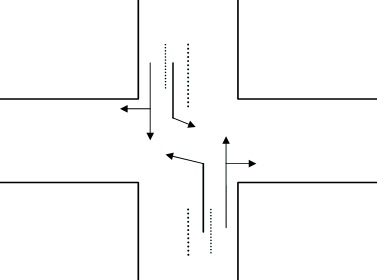
\includegraphics[scale=0.4]{simple_intersection.png} 
\end{center}
\label{fig:simple_intersection}
\caption{Simple intersection}
\end{figure}

Thus a specific phase $p = p_n(t) \in \lbrace 1,...,P_n \rbrace$ is selected for each timeslot. With this definition the green splits are implicit in the phase sequence. 

Now $\Psi = \lbrace \textbf{p} \rbrace $ and we can perform an optimization.

Satisfaction of minimum and maximum green times is the most common constraint, usually defined within a cycle. In this model the following equation must be satisfied:

$$
\forall p,n: \; T = \lbrace t: p_n(t) = p \rbrace \; st. \; cons(T) \wedge T_{min,p,n} \leq |T| \leq T_{max,p,n} 
$$
Thus $T$ is a set of points in time and the $cons$ function is defined by:
$$
cons(T) = 
\begin{cases}
true & if \;  \displaystyle\sum_{t \in T}{t} = � \cdot (\max T + \min T) \cdot (\max T - \min T + 1) \\
false & otherwise
\end{cases}
$$

That is, there must be a consecutive series of time slots (tested by using the Gaussian formula) in which phase $p$ is run.

\section{Types of Traffic Signals}
\label{sec:signal_types}

At present there are three major types of traffic signal systems
called {\em pretimed signals, actuated signals and adaptive signals}. They
are the result of incremental improvements described in chronological
order below:

\begin{description}
\item[Pretimed] signals uses static plans for phase sequences, cycle time and green splits according to the day of time. 
\label{insec:pretimed}
They are based on the assumption that demand is fairly stable within
certain divisions of time eg. morning, midday and evening or workday /
weekend. For instance, in the morning (7am to 8.30am) and afternoon
(15.30pm to 17.00pm) the traffic is usually heavier than during the
day or night due to the commuters.

Traffic may prove to be more dynamic, though, and therefore the
utilization of these signals must be monitored on a regular basis so
proper adjustments can be made.

\item[Actuated] signals function like pretimed signals but with the ability to \textit{lengthen} the green period with a certain amount, if additional vehicles are observed. 
\label{insec:actuated}
To achieve this the signal needs detector input about the demand it
faces for each phase.

A major disadvantage due to the autonomous operation is that it
becomes impossible to setup green waves since signals start their
cycle at arbitrary offsets and are unlikely to share a common cycle
time.

\item[Adaptive] signals is a network of signals which attempts to
optimize some MOE in an manner which is at least as intelligent as for
actuated signals.

The key to adaptive signals is reliable detection and short term
prediction of traffic. Adaptive signals must be able to respond to the
dynamic aspects of traffic, which are not captured in the design of
pretimed signal plans. Adaptive signals use historical input and
current detector input to make short term predictions for what is
going to happen eg. within the next minute, next 10 minutes and so
forth.

For this reason, and as stated in \cite{1}, adaptive systems are not
truly adaptive because they rely on these short term predictions and
thus will always lag behind the actual traffic. For short term
prediction methods from time series analysis eg. ARIMA models (see
eg. \cite{shortpredict}) can be used to get more accurate
predictions.

An isolated adaptive signalized intersection has advantages over
actuated signals because it can skip a phase to give priority to a
bus, for instance. The main attraction with adaptive signals is when
they can be set to work together. A good system will naturally cause
green waves to appear and move the direction of the green waves along
with changes in flow.
\end{description}

%\section{Traffic Detection}
%\label{detection}
Detection is the Achilles' heel of adaptive traffic control systems. An otherwise perfect prediction algorithm will provide flawed information to the optimization procedure, if sensors are misplaced or there are too few of them. Even with a dense sensor network lag issues may cause problems in the prediction and timing.

In Copenhagen upstream sensors are connected to the approaching signal controller which relay data to an area-specific hub, which is monitored by a central computer. Most of the signals are transmitted via cables, which are often severed by entrepreneurs so wireless, IP based alternatives are being explored.

The most common type of sensor in the areas supervised by Centre for Traffic and the Danish Road Authority is the induction loop. It is set into the tarmack and gives an indication whenever a metallic object (vehicle) passes. To detect buses extra large loops, which can only be triggered by large vehicles, are used. 

These authorities also use video detection and radar. Video is relatively cheap and can be installed without obstructing the traffic. Radar functions a bit like video but is more reliable under bad weather conditions and gives depth information.

Video is the most promising detection technology due to its rapid development and the possibility to perform post-processing on a computer to obtain additional informations besides vehicle detection. For instance, video images are being used in Copenhagen to measure travel speeds (a MOE). This is done by reading parts of license plates at point A and measuring the time for it to reach some other point, which is filmed.

\section{Milestones of Traffic Signal Optimization}
\label{history}
Some of the first public research into the optimization of traffic signals was published by Wardrop \cite{Wardrop} and Webster \cite{Webster}. Wardrop determines the Stochastic User Equilibrium essential for network assignment and the prediction of demand. 

\subsection{Delay and Queue Models}
Proper estimation of delays at an intersection is important in the design of signal plans.

Webster gives an approximate formula for average delay for isolated intersection with a fixed timing plan under steady state and undersaturated conditions ie. the flow cannot be dynamic and the inflow. 
He uses his own result to give expressions for the optimum cycle- and green times. 
Websters results have been widely used in the litterature eg. in \cite{1} to generate initial solutions of cycle length and green splits for a metaheuristic search and in \cite{30} to calculate cycle lengths.

The problem with Websters delay formula, along with other delay formulas developed from queuing theory is the assumption of steady state conditions. As the load on the intersection increases it will take longer time to reach stochastic equilibrium \cite{traffictheory}. During the stabilization period the signal settings must remain fixed, which it will never be in adaptive systems. These types of models are still used see eg. \cite{38} where Mirchandani and Zou develops a FIFO single-server queueing model with Poisson arrivals.

Time series analysis and other \textit{moving average} techniques can be used to relax these assumptions. In \cite{shortpredict} an ARIMA process is used to make short term (1 minute) predictions of arrivals. The RHODES system \cite{44} makes short term predictions on multiple levels of resolution (single-vehicle and platoons). In \cite{1}                                                                                          a Poisson process is used to calculate the interarrival time, with the parameter being the mean arrival rate thus anticipating the dynamic nature of traffic.

\subsection{Traffic Assignment}
Traffic signals are set to accommodate the flow of traffic thus it is vitally important to \textit{know the flow} in advance. Wardrop contributed with two principles concerning traffic flow:

\begin{enumerate}
\item \textbf{User Equilibrium:} (UE) each trafficant has minimized his own travel time (greedy route choice)
\item \textbf{System Equilibrium:} (SE) the average travel time is minimized (coordinated route choice)
\end{enumerate}

Given the choice a user will select the route which he \textit{perceives} to be the best. This route does not necessarily correspond with the actual shortest route, which has led to the Stochastic User Equilibrium (SUE) variation where this error is modelled by a stochastic element. 

The SUE is the most realistic model since 1) trafficants may not have perfect route information and may also choose a longer route on purpose (for the scenery, eg.) and 2) trafficants, at present, cannot communicate in order to obtain SE. In addition the SE entails that some trafficants may not have an optimal route, this kind of sacrifice will be difficult to accept.

In order to perform a traffic assignment for a network flow data is obtained from traffic counts or detector input over a time period. Auxilliary informations such as turning directions and vehicle types are collected as well, if possible. 

This data is fitted by a stochastic process and the optimization is made on the assumption that the process can describe the actual arrivals.

Thus there are two problems 1) determining demands and 2) optimizing the traffic signals accordingly.

It is important to realize that changing the traffic signal settings will cause changes to the flow and that changing the flow should cause the signals settings to be recalculated. This has given rise to a number of papers considering the two problems at the same time in so-called bilevel formulations eg. 
\begin{itemize}
\item \textbf{\cite{mc}:} iterative procedure which optimizes traffic signals and then solves the traffic assignment problem untill mutual consistency (convergence) is acheived
\item \textbf{\cite{34}:} gradient projection method for finding local optima combined with a global heuristic search
\item And in \textbf{\cite{2}} using a genetic algorithm approach.
\end{itemize}

A feature of adaptive systems is that they are less dependent on a large database of historical flow data since they use online data input from detectors, which they are, in turn, more dependent on. Thereby they do not have to consider the problem of mutual equilibrium between signal settings and user equilibrium.

\subsection{Optimization Methods and Architectures}
The surveyed articles span the period from the 60's to present. There are some tendencies which has been observed with respect to optimization methods.

A pattern for the earlier work seems to be the presentation of a mathematical model, which optimizes for one or more of the parameters mentioned in section \ref{theproblem}. The problem is then shown to be time consuming to solve using current computers and a heuristic is presented, which can cut down on the search space eg. by using "common sense" rules such as pruning of short cycle lengths under high saturation.

Later on the same models begin to become solvable by standard optimization packages due to advances in computer power as well as in the packages themselves.

\section{Systems for Offline Optimization}
\label{sec:offline}

The surveyed articles span the period from the 60's to present. In
this section some tendencies for offline optimization systems are
surveyed.

Most authors choose to present a mathematical model of the problem, in
the spirit of the one presented in section \ref{sec:model}, which
optimizes for one or more of the parameters mentioned in section
\ref{sec:theproblem}. Attempts to produce a closed-form solution for the
problem are seen often eg. \citet{36}, which presents a general model
that has resemblances with the model in section \ref{sec:dynamicmodel}.

For representation of network layout, the models are based on either
graph theory or some kind of cell transmission scheme or petri net
system. The petri net representation is very popular and some examples
of its use are \citet{12}, \citet{16} and \citet{petri}.

In a petri representation of a traffic network, spaces on links are
represented by cells, which can fit a single vehicle. When a cell is
occupied no other vehicle may enter. Vehicles progress through the
network by making transitions to adjacent cells. The stop-bars of
intersections can be represented in the petri net as a line of cells
blocking a link facing the intersection. When the phase begins the
stop-bar cells are enabled and vehicles may pass.  The petri net
representation fits well into the context of traffic networks due to
its representation of concurrency (spaces in a lane) and triggered
actions (cross on green light).

For the model to be solvable without an external evaluation tool, such
as TRANSYT, it must contain functional constraints which relate
eg. the proper offset for signals along an arterial to flow-specific
parameters such as saturation flow rate and the platoon dispersion
factor.  The model must also adjust link flows according to the signal
settings, that is, the model must be bilevel, as introduced in section
\ref{sec:bilevel}. An example of such a model is seen in \citet{33} where a
genetic algorithm finds optimal signal timing plans, considering user
response to signal changes. TRANSYT is used to obtain a fitness (MOE)
value and the Path Flow Estimator for determination of the stochastic
user equilibrium.

Considering a typical optimization formulation involving a common
cycle time, green splits and offsets, it is clear that - even with some
discretization of time - the search space is vast, especially when
considering some form of simulation for obtaining the objective
value. An example of a heuristic designed to cut down the search
space is ADESS (see \citet{26}). Most often the heuristics are embedded
into the search routines and operate, for instance, by using "common
sense" rules such as pruning short cycle lengths under high
saturation or by exploiting sensitivity knowledge of the problem
\citet{40}.  Another way to deal with this issue is to employ a
metaheuristic search, which is simply run until a result is
needed. Some examples are: \citet{1} (tabu search), \citet{42} (particle
swarm optimization) and genetic algorithms, which are the most popular
metaheuristics, by far see \citet{13}, \citet{33}, \citet{43}, \citet{7},
\citet{41}, \citet{31}, \citet{27}, \citet{2} and \citet{26}.

Systems which operate in this manner are mostly suited to offline use
considering that some reported running times are as high as several
hours, even for small networks.  Some authors eg. \citet{16} turn
such a system into an adaptive system by re-running the optimization
procedure every $K$ cycle but clearly this strategy is not possible
for systems with long run time requirements. Furthermore the next set
of signal timing settings may be quite different from the current one
and changing plans in an instant will cause transient sideeffects such
as malfunctioning green waves.

Much work focuses on optimizations for single intersections or
coordination of signals along an arterial. Gartner et al. \citet{9}
gives a walkthrough of the most promising progression schemes at the
time (PASSER-II, NO-STOP-1) and extends the MAXBAND approach from a
single-arterial bandwidth optimization into MULTIBAND, which optimizes
bandwidth along multiple, possibly intersecting, arterials. \citet{6}
is an example of the selection and optimization of an arterial - or
priority route - with subsequent network-wide optimization, taking the
arterial optimization as a constraint.  In the article \citet{24}
Heydecker propose how to use existing optimization methods for single
intersections in combination to achieve a network optimization. Though
Heydecker admits that, because of the decentralization, it will be
difficult to obtain coordination.


\section{Adaptive \& Cooperative Systems}
\label{sec:adaptive_cooperation}

Adaptive traffic control systems aim to coordinate signal controlled
intersections so as to optimize some performance index eg. average
delay or number of stops (or a combination) but also to reduce the
need for constant supervision and tuning of intersections.

They do this by dynamically adjusting cycle times, phase sequences and
green splits according to traffic detected as well as the predicted
traffic, thereby reacting to those dynamic aspects of traffic,
which cannot be captured by the static optimization routines used to
generate time-of-day plans. Some authors (\citet{1}, \citet{44},
\citet{46},
\citet{scoot2004}) even skip or work around the conventional periodic
scheme based on a common cycle time and make direct assignments of
phases and allow phases to be skipped, as presented in section
\ref{sec:dynamicmodel}.

It is evident that the cycle time is crucial in optimization because,
for a congested network, increasing the cycle time will always cause a
throughput increase (there are always cars waiting to cross the
intersection). In the literature the cycle time is often common to
all intersections under traffic control so that green waves (arterial
progression) can be produced. For direct assignment systems the
throughput is dependent on allocation to phases of consecutive green
time. Long cycle times lead to long phase durations, which allow a
steady flow of vehicles to pass and minimize lost and interphase time
per time unit.

For large networks the enforcement of a common cycle time is
inappropriate, however. Consider a network which is so large that two
disjoint arterials exist. In this case it is unlikely that a common
cycle time will allow green waves to exist for both arterials. For
networks of this type (size) a direct phase assignment model might
provide the necessary flexibility. Another feature of considering very
large networks is the possibility of traffic redirection. If it is
detected - or predicted - that an arterial is, or will be, congested
under current flow conditions it is sensible to redirect some traffic
onto alternative routes.

In this section some in-depth discussions are given for three adaptive
systems, which do not rely on offline optimization as it was presented
in section \ref{sec:offline}. The systems are:

\begin{enumerate}
\item \textbf{RHODES} by Pitu Mirchandani and Larry Head presented in
\citet{44} - a hierarchical system for network-wide optimization.

\item A \textbf{Phase-by-Phase} optimization strategy by Michael
Shenoda and Randy Machemehl presented in \citet{1} - a system using the
metaheuristic tabu search for determining greens for isolated
intersections in a phase-by-phase manner.

\item \textbf{DOGS} by Danish Technical Traffic Solution (TTS)
evaluated in the Danish article \citet{dogs}, which provides
criteria-based capacity increases along an arterial.

\end{enumerate}

The systems will be compared in the areas of \textit{prediction} and
\textit{optimization strategy}.

\subsection{RHODES}
\label{sec:rhodes}

RHODES approach to traffic signal optimization is a hierarchical one
with 3 layers of detail, see Figure \ref{fig:rhodes_hierarchi}.

The macroscopic layer performs \textit{dynamic network loading}, which
involves observing changes in the aggregated flow data of the entire
network due to variations in the OD matrices. This layer supplies
estimates of link flows to the middle level in rough numbers
eg. vehicles per hour.

The mesoscopic middle layer considers sectors of the network eg. an
arterial. This \textit{network flow control} layer work in the detail
level of platoons and average speeds. Green time is allocated to
phases to accommodate the movements of the platoons and so
coordination of intersections is done at this level.

At the lowest level is \textit{intersection control} where vehicles
are handled individually (a microscopic layer). Here the green times
and phase ordering suggested by the middle layer are fine tuned.

\begin{figure}[!ht]
\begin{center}
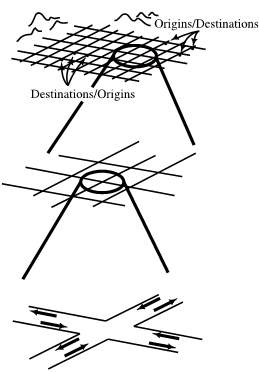
\includegraphics[scale=0.5]{rhodes_hierachy.png} 
\end{center}
\caption{The three levels of detail: network, sector, and intersection}
\label{fig:rhodes_hierarchi}
\end{figure}

An adaptive traffic control system must operate quickly in order to
adapt signals to traffic in real-time. The RHODES platform has good
decomposition opportunities and is pluggable ie. the upper level is a
black box feeding the lower level with predictions and
optimizations. At the time the article was written, the top level of
RHODES had not received much development and thus only the middle and
lower level are described herein.

\subsubsection*{Detection}
Detection methods are not discussed in detail in the paper. They can
be of any technology including induction loops and video.

\begin{figure}[!ht]
\begin{center}
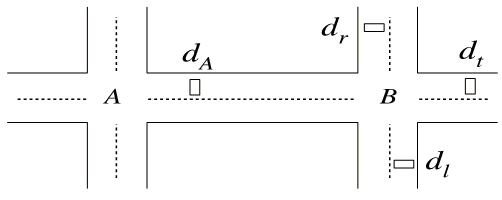
\includegraphics[scale=0.5]{rhodes_prediction-strategy.png} 
\end{center}
\caption{Detector placement and propagation of information in a simple grid}
\label{fig:rhodes_predict}
\end{figure}

\subsubsection*{Prediction}
The PREDICT method by the co-author, XXX Head 1995 XXX, is used to make
predictions for individual vehicles. PREDICT is built for network
prediction and relies on the fact that incoming flow to an
intersection originates from adjacent intersections. This concept can
be explained from Figure \ref{fig:rhodes_predict} where traffic
detected at $d_a$ is the sum of right-turning traffic at detector
$d_r$, left turning traffic at $d_l$ and through-going traffic at
$d_t$.

Thus given flow estimates for the links facing intersection B and
turning probabilities for each link an estimate can be given for the
inflow to intersection A from east. On the link between the two
intersections there will be traffic entering and exiting the system,
but these contributions - and losses - to the traffic, which can be
measured at $d_a$, are expected to be very small.

Prediction of arrival times of the vehicles which has passed detectors
$d_{\lbrace r,t,l \rbrace}$ depend on the current phase at
intersection B and queue conditions. Mirchandani and Head has
identified four cases, which cover arrivals to an intersection, which
are summarized in table \ref{tbl:delaycases}.

\begin{table}[!ht]
\begin{center}
\begin{tabular}{l|ll}
 & \textbf{Green} & \textbf{Red} \\ \hline
\textbf{No queue} & 0 & $T_G$ \\
\textbf{Queue} & $T_Q$ & $T_G$ + $T_Q$
\end{tabular}
\end{center}
\caption{Delay incurred for a vehicle arriving to an intersection in various states where $T_Q$ is the time for ahead queue to clear and $T_G$ is the time to the next green.}
\label{tbl:delaycases}
\end{table}

In the cases involving queue there is, of course, a possibility that
the vehicle will not be able to cross the intersection before several
green phases have occurred. This is likely to happen under high
congestion when intersections are placed closely.

At the mesoscopic level, network flow control, the APRES-NET
prediction method is used. It is based on simulation and has
similarities to PREDICT, though it works in the detail level of
platoons and encompasses several intersections, not just the upstream
ones but also those upstream of the upstream intersections and so
on. Since the 2nd level must deliver complete suggestions for timing
plans for each intersection (to be fine tuned by intersection control)
it must run quickly. Performance is dependent on the number of
intersections in the monitored sector and sector sizes can thus be
scaled to match the speed requirements depending on hardware.

The prediction horizon for network flow control is 200-300
seconds. Cycle times for simple intersections with just a couple of
phases vary between 60 and 150 seconds so this horizon is plenty to
predict and respond to most types of fluctuations by performing phase
skipping, phase reordering and assignment of phase durations. The
intersection level control operates with a prediction horizon of 20-40
seconds and thus can only make decisions on whether to lengthen or
decrease the green time of phases within that horizon.

\subsubsection*{Optimization}
As in the dynamic model of section \ref{sec:dynamicmodel} timing plans are
described by phase ordering and duration independent of cycle time,
splits and offsets.  Optimization is performed on each level using
prediction results for that level.

At the network flow control level the REALBAND algorithm forms
progression bands (ie. \textit{green waves}) for platoons traversing
the sector based on the predictions from APRES-NET. This is done by
finding \textit{conflicts} between platoons, which will request access
for conflicting phases at the same time. In this way a conflict can be
regarded as the denial of green to a platoon due to the passage of
another platoon. A decision tree within the optimization horizon of
200-300 seconds is build and explored to find the configuration with
the fewest conflicts. This results in a set of phase orderings and
green times for each intersection.

At the lower level a dynamic programming approach, COP, takes the
results from REALBAND and distributes green time for some horizon to
the phases received from the above level. The phases and their
ordering must be respected so as to not introduce conflicts, which
have been resolved by REALBAND. For the same reason there are
restrictions for the maximum change in either direction of the given
green times, but COP is allowed to use its more detailed predictions
to perform the mentioned fine-tuning of green times.

\subsubsection*{Evaluation}
RHODES has been implemented and evaluated in CORSIM as part of the
evaluation for Federal Highway Administration (FHWA) inclusion in
RT-TRACS. RT-TRACS is an effort to choose and standardize a peak
performance traffic signal optimization system for American traffic
networks.

The simulation is done for an arterial of 9 intersections with steady
increase and then decrease of traffic over a 2 hour period. This is a
FHWA test case and the baseline traffic control system is
semi-actuated control based on the results of offline tools including
TRANSYT and PASSER, which represents the best-can-do from an offline
approach and can be considered a hard competitor.

Testing shows that RHODES is more capable of exploiting the capacity
of the arterial. As long as there is no congestion the throughput will
match the demand and in the comparison RHODES can simply take more
load before experiencing congestion.

Real adaptive systems should excel in the case of low demand, since
the overcapacity will then allow RHODES to, roughly said, cater for
each vehicle. The effect, compared to the semi-actuated control, is
convincing with 50\% reduction in delays for low demand and 30\%
reduction for high demand. This effect is expected to disappear when
demand reaches the capacity of the arterial in which case, for both
systems in the comparison, only throughput can be improved by
increasing the green time along the arterial and maintaining proper
coordination.

The simulation was run multiple times and for both throughput and
delay it is clear that RHODES is more consistent than semi-actuated
control and offers less variability from run to run.


\subsection{Phase-by-Phase}
The phase-by-phase (PP) system was developed to overcome a number of deficiencies, which seemed widespread in adaptive systems:

\begin{itemize}
\item Fixed cycle length and/or fixed step for variation of cycle length
\item Utilization of aggregated demand data only
\item Fixed coordination of signals along an arterial og through a network
\end{itemize}

The proposed overall scheme to improve upon these issues are the isolated optimization of intersections and more fine-grained tracking of vehicles.

The optimization process has been made independent from determination of the network state ie. detection and prediction and as such some of these subjects are mostly discussions and proposals for improvements.

\subsubsection*{Detection}
PP relies on individual tracking of vehicles to obtain an arrival based model. For networks this can be realized only with video detection with eg. license plate recognition; traditional loop detections cannot yet identify individual vehicles.

The PP system currently works for isolated intersections and so detection loops are sufficient to estimate arrival times. For detector placement, the authors suggest using simulation.

\subsubsection*{Prediction}
In the proposed form the PP system uses a Poisson process to generate interarrival times.
Alternatives are some form of time-series analysis or a Poisson process with variable mean. The use of detections made upstream could also be used, such as it is in RHODES.

The performance of PP is highly dependent on the ability of the chosen prediction system to generate proper forecasts but, as will be seen in the test results, the potential benefits are great.

\subsubsection*{Optimization}
The optimization procedure of PP seeks to minimize the stopped delay using input from the prediction process. The most widely used measure of effectiveness is stopped delay (see eg. \cite{9}, \cite{38} and \cite{31}) but the authors show that there is also a linear relationship to total travel time.

The following notation is used in the paper:

\begin{table}[!ht]
\begin{center}
\begin{tabular}{ll}
\hline
$H$ & Horizon of optimization \\
$cs$ & Cycle start time \\
$ce = cs+H$ & Cycle end time \\
$i = 1,...,N$ & Approach indexes \\
$k = 1,...,M$ & Phase indexes \\
$\lambda_k$ &  Is a partitioning of $H$ into phases and $0 = \lambda_{0} <  \lambda_{k-1} \leq \lambda_k \leq 1$ \\
$\lambda_{k_i}$ & The time into $H$ before the phase $k$, involving approach $i$, ends \\
$j$ & Vehicle id for predicted vehicle arrival within the horizon  \\
$t_{ij}$ & The arrival time for vehicle $j$ on approach $i$
\\ \hline
\end{tabular}
\end{center}
\caption{Notation}
\end{table}

$H$ should be in the order of the desired cycle time and $\lambda_k$ give the green splits and thus we have a full plan for the signal. Stopped delay can be calculated from this plan and the predicted arrivals. In Figure \ref{fig:pp_delay} this idea is sketched.

\begin{figure}[!ht]
\begin{center}
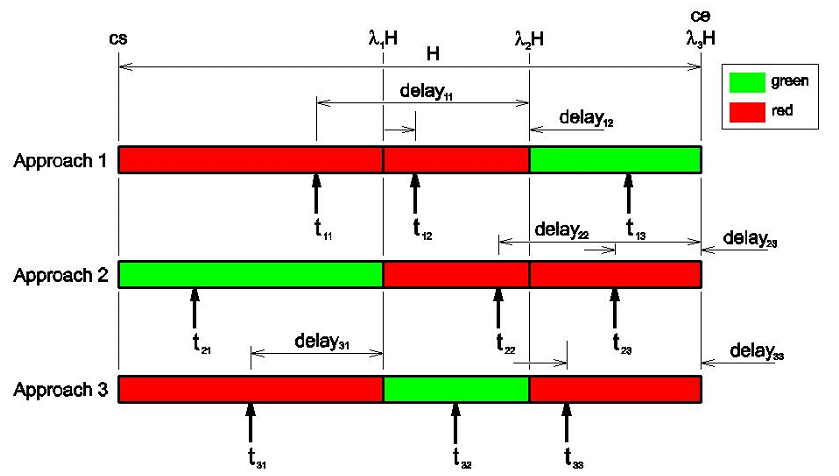
\includegraphics[scale=0.5]{phase-by-phase_delay-model.png} 
\end{center}
\caption{Calculation of stopped delay in the Phase-by-Phase system for an intersection with 3 approaches and 1 exit (no turning movements).}
\label{fig:pp_delay}
\end{figure}

In equation \ref{eqn:pp_delay} the rules for stopped delay are extracted when vehicle $j$ arrives on approach $i$ at $t_{ij}$.

\begin{equation}
delay = 
\begin{cases}
cs + H \cdot \lambda_{k_i-1} - t_{ij} & when \; t_{ij} \leq cs + H \cdot \lambda_{k_i-1} \; (before\;green)  \\
cs + H - t_{ij} & when \; t_{ij} \geq cs + H \cdot \lambda_{k_i} \; (after\;green)  \\
0 & otherwise
\end{cases}
\label{eqn:pp_delay}
\end{equation}

In the second case of equation \ref{eqn:pp_delay} vehicles incur stopped delay since they arrive after their approach has been served green time in the planning horizon. Thus they will not be served before the next green, which has not yet been planned, and stopped delay is accumulated until then. This is called carryover since vehicles are carried over into the next cycle.

PP also takes into account queue startup delay and thus cover the most critical sources of delay. However PP makes the assumption that the granting of green time to a phase will cause the approaches to be cleared completely ie. no vehicles must experience more than one green phase before they can leave.

The objective function is defined using these delay terms and thus optimization can be done by making changes in the $\lambda_k$-values within some critical points in horizon. Looking at Figure \ref{fig:pp_delay} it is seen that approach 2 is served green time until $\lambda_1 H$, supressing green from approach 1 and 3, which both have arrivals. By switching phase immediately after $t_{21}$ (setting $\lambda_1 = (t_{21} - cs)/H$) approach 1 could receive green until immediately after $t_{12}$ and so on. This example involves switching of the phase order, which was turned off in the paper.

In the PP paper \cite{1} a solution method using the above scheme is presented as a combinatorial problem. But the number of combinations increase exponentially with the number of arrivals and the number of phases. Therefore a tabu search is employed. Websters formula for optimum green time splits is used in the Proportional Heuristic to obtain a good initial solution and a 1-bit neighborhood function is defined by making changes to a single value in $\lambda_k$ (a low influence move), preserving the phase order. Candidates for the step of these changes range from the transmission time of an electronic signal ($\approx 10^{-3}s$) to the minimum headway between two vehicles travelling in a platoon ($\approx 2s$ cf. Greenshields et al. 1947).
A high influence move, which reorders phases, is also described but is turned off, as mentioned.

\subsubsection*{Evaluation}
Shenoda and Machemel compares the results of their metaheuristic search to pretimed and actuated signal control settings obtained from the CORSIM microsimulator using the test intersection in Figure \ref{fig:pp_intersection}.

\begin{figure}[!ht]
\begin{center}
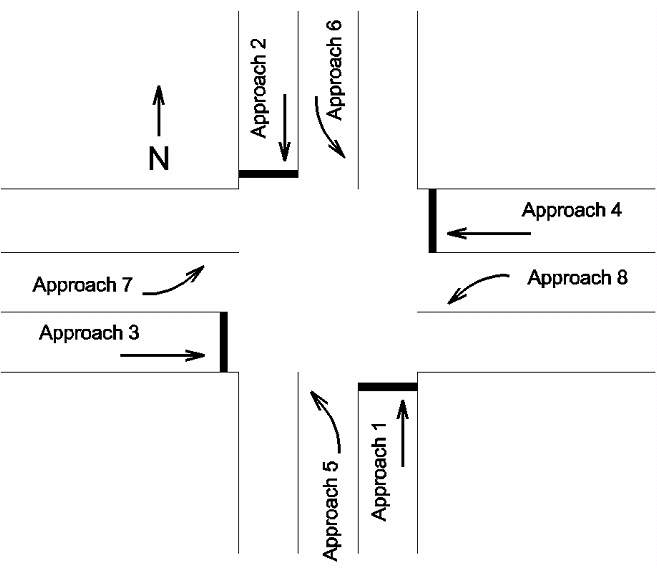
\includegraphics[scale=0.5]{phase-by-phase_testing-intersection.png} 
\end{center}
\caption{4-phase intersection from experiment \#2}
\label{fig:pp_intersection}
\end{figure}

The intersection was subjected to 8 different data sets of arrival times. In Figure \ref{fig:pp_improvements} the stopped delays for the PP system is compared to the simulation results using pretimed plans and standard traffic actuated control.

\begin{figure}[!ht]
\begin{center}
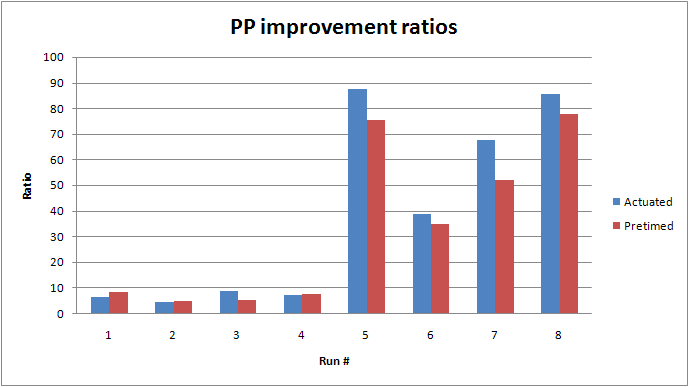
\includegraphics[scale=0.5]{phase-by-phase_improvement_ratios.png} 
\end{center}
\caption{Improvement factors of PP compared to pretimed and actuated control in the 4-phase intersection of Figure \ref{fig:pp_intersection}}
\label{fig:pp_improvements}
\end{figure}

The results should only be taken as indications since a number of assumptions were made for PP that the prediction algorithm supplied perfect information. In addition the actuated control was only semi-actuated since detectors were only used in one direction, the other being timed as in the pretimed case, which was optimized using Websters formulas.

In spite of these issues it is interesting to observe the the (semi-)actuated control strategy is not always superior to pretimed plans. It is clear, however, that both strategies are outperformed by PP. Under the given assumptions - in particular that concerning accuracy of predictions - PP can be used to establish a baseline for the best possible performance. This becomes even more true when the phase ordering constraint is dropped allowing reordering and skipping of phases.

Unfortunately Shenoda and Machemehl do not test PP on a network or even along an arterial. The optimization procedure does not consider coordination in itself though it is proposed that the prediction routine should consider departures from adjacent intersections, such as the method by Head employed in RHODES. It is speculated that such propagation of departure information could give rise to some coordination, depending on the horizon of optimization.

\subsection{DOGS}
\label{sec:dogs}

DOGS is an extension of the DOG system. The first 3 letters can be
directly translated from danish to \textit{dynamic optimization of
greens} and the appended S of the herein regarded system means
\textit{coordination}. Thus DOG is an traffic actuated optimizer for
single intersections, as described in section \ref{insec:actuated},
and DOGS add coordination. The DRD has implemented DOGS along several
arterials in Denmark.

DOGS is a criteria-based system which relies on a common cycle time
for coordination. The intended area of application is traffic signals
along arterials, which see a high fluctuation in demand.

The purpose of DOGS is to increase the capacity of the arterial in
high demand periods and revert to offline-optimized, pretimed plans in
low traffic situations. The capacity increase is realized by
increasing the common cycle time and allocate the extra green time per
cycle to the phases along the arterial. This will cause increased
delays for the minor roads, but may prevent queues from reaching the
previous intersection - or even prevent queues in cases of light
congestion.  DOGS is also capable of providing priority to buses by
extending the green time when buses are near an intersection.

At present the system must be tailored to the environment in which it
operates. For this reason the following sections will use the Herlev
area in Denmark as a reference area in order to explain certain
concepts. In Figure \ref{fig:dogs_herlev} is a layout of this network.

\begin{figure}[!ht]
\begin{center}
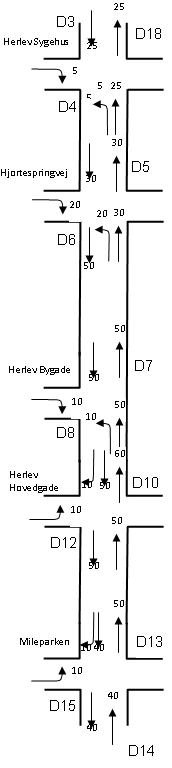
\includegraphics[scale=0.5,angle=90]{dogs_herlev.png} 
\end{center}
\caption{Layout of the partial O3 arterial in Herlev, which is under DOGS control. The arrows and numbers indicate flow direction and examples of typical vehicle count.}
\label{fig:dogs_herlev}
\end{figure}

\subsubsection*{Prediction}

DOGS is a purely traffic actuated system and no prediction is used
when the system is activated due to heavy traffic conditions.
In spite of the intended flexibility of the system this is a point
which puts high demand on the implementing traffic engineers since
traffic through the arterial must be assessed manually when the system
is put into production as well as during maintenance.

An alleviating point to the lack of prediction is the fact that the
current arterials under DOGS control are relatively small and static
predictions can be made by an experienced traffic
engineer. Furthermore, since DOGS only operate under high load
conditions, predictions become less valuable - or superfluous, even -
because all that can be said about the arterial in this case is that
it is heavily loaded with traffic.

\subsubsection*{Optimization}

Since DOGS only kicks in under congested or near-congested conditions
(for the Herlev area when the load exceeds 60\%) it is simple to
optimize the throughput since any increase in green time will just
allow more vehicles to pass (the phase is never emptied from
vehicles).

That DOGS only operates during high-congestion levels is an unusual trait for an adaptive system since they usually excel in optimization under \textit{normal} ie. uncongested load conditions (see the comparison of RHODES and a semi-actuated system in section \ref{sec:rhodes}). This can be explained from the lack of an explicitly defined objective function and optimization routine.

The objective is to keep the load degree (load/capacity) for the most heavily loaded intersection below 90\%.
To do this the common cycle time and green times are set according to the load level. The adjustments are made with a few seconds per cycle to avoid sudden, major changes in cycle time and temporary loss of coordination.

Coordination is achieved by running the signals on a common cycle time, but offsets are not adjusted when the common cycle time changes so this issue should receive further investigation.

A set of non-overlapping criteria are used to select a program with the appropiate capacity for the detected inflow. For a technical description of these criteria cf. \cite{forprojekt}

%% When naming the inflow detectors in the north- and south ends $DN$ and $DS$, respectively, the transition from pretimed control to adaptive control is decided by the constraint:
%% \begin{eqnarray*}
%% Intensity(DN) > I_{enable} & \vee & Intensity(DS) > I_{enable} \\
%% & or & \\
%% Load(DN) > L_{enable} & \vee & Load(DS) > L_{enable}
%% \end{eqnarray*}

%% For switching back to pretimed control this constraint must hold:
%% \begin{eqnarray*}
%% Intensity(DN) < I_{disable} & \wedge & Intensity(DS) < I_{disable} \\
%% & and & \\
%% Load(DN) < L_{disable} & \wedge & Load(DS) < L_{disable}
%% \end{eqnarray*}

%% To avoid hysteresis ie. constant enabling and disabling of dynamic control:
%% \begin{eqnarray}
%% I_{enable} - I_{disable} & \geq & I_{\varepsilon} \label{eqn:hysteresis_intensity} \\ 
%% L_{enable} - L_{disable} & \geq & L_{\varepsilon} \label{eqn:hysteresis_load} \\
%% I_{\varepsilon},L_{\varepsilon} & > & 0 \label{eqn:hysteresis_limits}
%% \label{eqn:hysteresis}
%% \end{eqnarray}

%% DOGS exhibits a dynamic behaviour because the permitted cycle time extensions are divided into \textit{programs} according to the intensity and load levels in the ends of the artery. These program constraints take a form which is similar to the enable- and disable constraints.

%% When deciding whether to remain in the current program, $i-1$, or switch to a program for higher demand, $i$, the following relation must be satisfied:

%% \begin{eqnarray*}
%% I_{enable,i+1} \geq & \max(Intensity(DN),Intensity(DS)) & > I_{enable,i} \\
%% & \vee & \\
%% L_{enable,i+1} \geq & \max(Load(DN),Load(DS))  & > L_{enable,i}
%% \end{eqnarray*}

%% The decision of switching from program $i$ to the program for lower demand, $i-1$, is determined by this relation:

%% \begin{eqnarray*}
%% I_{disable,i-1} \leq & \max(Intensity(DN),Intensity(DS)) & < I_{disable,i} \\
%% & \wedge & \\
%% L_{disable,i-1} \leq & \max(Load(DN),Load(DS))  & < L_{disable,i}
%% \end{eqnarray*}

%% In the DOGS controlled area in Herlev there are 8 different programs to choose from and the enable and disable thresholds for programs respect the ordering implicit in the above equations:

%% $$\lbrace I,L \rbrace_{enable,i+1} > \lbrace I,L \rbrace_{enable,i}$$
%% $$\lbrace I,L \rbrace_{disable,i-1} < \lbrace I,L \rbrace_{disable,i}$$

%% To avoid hysteresis between programs the same constraints (equations \ref{eqn:hysteresis_intensity}-\ref{eqn:hysteresis_limits}) as for switching between pretimed and dynamic control applies.

\subsubsection*{Evaluation}

Tests have shown that the system is indeed capable of increasing the
capacity, with reduced queue lengths as a result. When the arterial in
Herlev is at or above moderate load DOGS will increase the capacity by
15-25\% compared to the capacity if only the pretimed plans was in
use.


\subsection{Comparison}

The three systems presented here have different scope and as such
cannot be compared directly. The RHODES system is the most general,
being prepared for network-wide optimization, though it will perform
well along an arterial, as shown in the FHWA test case. The DOGS
system is specifically designed to increase capacity along an
arterial. It is very flexible but requires many input parameters, for
which there is no clear selection strategy. Finally the phase-by-phase
system performs advanced intersection control but had no inherent
strategy for coordination at the time this article was written.

Some comparisons can be made in the two main topics covered for each
system ie. \textit{prediction} and \textit{optimization}.

\subsubsection*{Prediction}

In this area RHODES is by far the most advanced system. The systems
used at intersection and sector level control and in the detailed
level and scope are similar and build on existing work. Predictions
are made from detector data from upstream intersections using turning
probabilities and speeds, which can be extracted from historical data.

At the time of writing, the Phase-by-Phase system had "perfect"
prediction ie. the prediction process was directly linked to the
traffic generation process of the simulator. The recommendation from
Shenoda and Machemel is to further investigate the ARIMA time-series
analysis framework to obtain accurate prediction for arrivals, which
they argue is of dynamic nature.

DOGS has no prediction capabilities. On the Herlev implementation
there is a general assumption that traffic which enters the arterial
at either end is assumed to pass through the arterial. Turn-in and
turn-out movements are thus expected to cancel out. This assumption
could prove to be cumbersome if DOGS was to operate on longer arterials
with differing traffic patterns in different regions.

\subsubsection*{Optimization}

DOGS has a clear advantage in optimization since, for each cycle, the
only decision to be made is whether to switch between traffic-actuated
control and pretimed signal plans or to change to a lower or higher
capacity program. This can be done in constant time using constraints
such as the one presented earlier. DOGS has no explicitly stated
objective function, only a \textit{political} objective - capacity
increase with reduced service for minor roads, which can be assessed
in rough terms using video detectors.

Phase-by-Phase minimizes delay using tabu search by adjusting green
time proportions assigned to phases. The initial solution is obtained
from a proportional heuristic, using Websters results, and the 1-bit
neighbourhood function redistributes the green time for one single
phase to the next.  The running time of the search algorithm can be
set to the maximum time before a decision must be implemented
eg. until the end of the current phase.

RHODES optimization in the middle level involves generation and
traversal of a conflict resolution tree in order to find the best path
ie. conflict resolution according to some MOE. The optimization is
made for predictions of traffic 200-300 seconds in the future. The
article on RHODES does not mention how often the middle level
optimization is performed, though it seems natural to reoptimize every
time new predictions become available or continuously, if they are
updated before the optimization completes.  The conflict resolution
timing plans are fed to the intersection level optimization, which
fine tunes the plans according to predicted arrival of individual
vehicles using a dynamic programming approach. The optimization is
valid for 45-60 seconds into the future and is rerun at the end of
each phase.


%\section{Simulation \& Evaluation of Solutions}
%\label{evaluation}
Until this point there has been no discussions of how solutions are evaluated. Fitness determination of a solutions is a major issue, especially in metaheuristic search, which put "blind faith" in the evaluation procedure. Furthermore the metaheuristic must evaluate a certain amount of solutions before confidence in the final solution is established, thus each evaluation must be fast, if the search is a part of an adaptive system rather than an offline optimizer.

There are two major methods for this evaluation. The first is based on the modelling of the complete system as a bilevel model (see section \ref{offline}) so that all necessary informations concerning signal states and traffic can be incorporated into the objective function. 

The second approach, simulation, handles the complexity issue of modelling the bilevel system and allows the modeller to rely on the simulation results as a black box for fitness evaluation. 

Simulation is widely used in the articles of this survey and so this section will discuss this method of evaluation.

There are a number of highly regarded simulations available. The primary use are for infrastructure expansions. In traffic signal optimization they are almost always used to establish confidence in performance for some signal optimization procedure. This confidence comes from observing the actions of the system during the simulation but also by comparing aggregated fitness values with those coming from some other, well-known approach. In this regard the TRANSYT offline traffic signal optimization package is often used as a baseline. 

In this case the quality of the simulation is more important than execution speed. 
In table \ref{tab:convergespeed} are the names of three major simulators, which are highly trusted to produce reliable traffic. 
From the interviews it emerged that the Danish Road Directorate prefer VisSim for simulations of infrastructure expansions as well as testing of signal timing plans. In the latter case also TRANSYT is highly regarded and will also perform much faster.

There are three types of simulators, the main difference being the level of detail in the underlying model. They are micro-, meso- and macrosimulators. Microsimulators model the behaviour of each vehicle and driver, mesosimulators regard the movements of platoons of vehicles and macrosimulators search for a user equilibrium (see section \ref{usereq}), considering origins (input links) and destinations (output links).

Independent on the detail level of the model a simulation must run until it is converged before the objective value can be extracted. 

Park et al. \cite{4} show that the CORSIM microsimulator is superior to the mesoscopic simulator from the TRANSYT package when combined with a genetic algorithm since the flow equations do not capture the dynamic aspects of traffic. But microsimulation is also slower to converge than the other types and thus evaluation of a solution will take longer. In a comparison study \cite{simcompare} Holst estimates the required simulation type as in table \ref{tab:convergespeed}.

\begin{table}[!ht]
\begin{center}
\begin{tabular}{c|c|c}
\textbf{VisSim} & \textbf{Dynameq} & \textbf{Time Slice Assistant} \\
\textit{(micro)} & \textit{(meso)} & \textit{(macro)} \\ \hline
1000 & 100 & 1
\end{tabular}
\end{center}
\caption{Estimate of of relative required simulation time for convergence}
\label{tab:convergespeed}
\end{table}

Microsimulation will not scale as well as meso- and macrosimulation since the number of vehicles in the network will grow in proportion with the total length of the roads. In mesosimulation the number of platoons need not grow as fast since some arteries traverse the entire network and a single platoon is regarded. The headway threshold for platoon definition could also be increased to compensate for the extra cars. Macrosimulators will scale in proportion with the size of the OD-matrices, which is the minimal level of detail and complexity for realistic results. 
Meso- and macro simulators, using deterministic principles, have another advantage since they can execute heuristic procedures to skip past much of the initial population of roads, which is mandatory in microsimulation when traffic begins to flow into the empty network. Since most simulations will be stopped whenever convergence is reached this is a very useful attribute.

For these reasons many of the surveyed articles use the mesosimulator of the TRANSYT optimization package. Some examples are \cite{26} which presents an improved metaheuristic search compared to the one which is built into TRANSYT-7F. In \cite{43} TRANSYT is extended so that there is no requirement of a common cycle time. The new model is used as a framework for testing adaptive systems with the TRANSYT simulator as a testbench.
In the last example Chiou \cite{34} generates solutions using a numerical search and tests them using TRANSYT.

Other researchers implement simple, but fast, microsimulators, for instance \cite{12} and \cite{42}. They are tightly coupled to the test network and their reliability is questionable.

In \cite{31} Taale and van Zuylen use a macroscopic simulator for evaluation solutions from their genetic algorithm, but recommend the use of a microsimulator for evaluation of the final solution. In spite of the macrosimulator they observe running times in excess of one hour for very small networks on current hardware. (This might also be due to poor tuning of the GA, but they do not mention this possibility.)

For microsimulations most often CORSIM is used eg.  \cite{1} and \cite{35}. Perhaps this is due to the fact that CORSIM is made by the same company, which sells TRANSYT - McTrans. A single use an alternative microsimulater, Paramics Quadstone, is seen in article \cite{21}.

The information that can be extracted from the simulators are plentyful for the purpose of comparing solutions to signal settings (delay, travel time, stops, queue lenghts). The articles presenting simulation results of seem to prefer microsimulations.

\section{Conclusion}
\label{sec:conclusion}

The emphasis of this survey has been on adaptive systems, which can
accommodate for the fluctuations in traffic.  The flexibility of the
model (or lack of it) underlying the optimization is a determining factor
regarding the level of adaptiveness that is achievable. The offline
optimization systems (section \ref{sec:offline}) all operate with the
common cycle time concept, which allows coordination to be set up by
offsetting downstream intersections. The common cycle time is
prohibitive when adaptive systems try to react to (predicted) arrival
of single vehicles or platoons of vehicles, even.

There are several models for traffic networks, which are not based
on the periodic behaviour of offline systems to perform
coordination. Instead they assign green time to phases in some order,
which is optimal given the detected and predicted traffic.  In section
\ref{sec:adaptive_cooperation} three systems were discussed in
detail. They were selected to give examples of adaptive control at
different levels (network, arterial and intersection). Two of them
(network and intersection control) use the direct assignment / phase
assignment methodology and the last (DOGS for arterial control)
operates with a classical model, but is designed so that the mentioned
problems are negligible.

DOGS is an example of a simple, but efficient, solution to dynamic
capacity adjustment for an arterial. It has been implemented for
multiple highway arterials and has thus proven that it can supply
capacity increases when needed as well as adjust priority to minor
roads once the traffic flow on the arterial diminishes.  DOGS has little
mathematical background, however, and has not been simulated prior to
implementation.  In a future project it would be interesting to
introduce a mathematical foundation for DOGS, preferably on the basis
on some established arterial progression scheme such as
REALBAND. Before and after scenarios could be simulated to determine,
what improvements are possible by going from a system adjusted by
ad-hoc methods to a truly optimized system.


\bibliographystyle{alpha}
\bibliography{bibfile,extra}
\end{document}
